\documentclass[11pt]{article}
\usepackage{amsmath, amssymb, graphicx, booktabs, hyperref, natbib}
\usepackage[a4paper, margin=1in]{geometry}

\title{Building Local-Language Economic Narrative Indices: \\
The BENI v1 Pipeline from Raw News to Validated Measurement}

\author{Ann Naser Nabil \\
Department of Economics, Jahangirnagar University \\
\texttt{lila.lab0x@gmail.com}}

\date{June 2026}

\begin{document}

\maketitle

\begin{abstract}
Economic narrative indices---monthly measures of economic news salience---are well-established for English-language media but remain scarce for low-resource languages. We present the BENI v1 method pipeline, a reproducible workflow for transforming Bangla-language news into economic narrative measurements for Bangladesh.

The BENI v1 database combines dated Potrika articles from 2014--2020 with post-2020 BNAD articles, producing 1,467,705 harmonised article records with source metadata, deduplication fields, economic seed labels, and model-ready text. The current frozen validation set contains 186 clean reference labels mapped to canonical BENI v1 article IDs; the remaining 114 ambiguous rows are conservatively excluded from clean validation.

In the frozen BENI v1 validation run, TF-IDF + Logistic Regression achieves 88.17\% accuracy, $\kappa = 0.736$, precision of 92.73\%, recall of 73.91\%, and F1 of 0.823 on the Economic class. The corresponding monthly BENI v1 index is built from 1,453,510 deduplicated article predictions and provides both article-weighted and source-balanced specifications.

The contribution is a complete low-resource measurement template: database harmonisation, weak labeling, LLM-assisted reference annotation, frozen validation, article-level prediction, index construction, and macro-validation checks. Legacy Potrika calibration results are retained as prototype evidence only; the final BENI v1 outputs are grounded in the repaired corpus and frozen validation set.

\textbf{Keywords:} economic narratives, Bangla NLP, low-resource text classification, annotation cost, narrative index, BENI

\textbf{JEL Codes:} C53, C55, E37
\end{abstract}

% Paper 3 — Introduction Section
% Building Local-Language Economic Narrative Indices

\section{Introduction}

Text-as-data methods have transformed empirical research in economics, political science, and sociology \citep{gentzkow2019text, grimmer2019text}. Researchers now routinely extract sentiment, topics, and narrative frames from news articles, social media, and policy documents to measure economic conditions, predict financial markets, and understand public discourse \citep{tetlock2007sad, baker2016measuring}. Yet this transformation has been overwhelmingly English-language: 84\% of published studies analyze English text, and 56\% focus exclusively on the United States \citep{nabil2026economic}.

This linguistic concentration creates a fundamental measurement gap. For the 5.5 billion people who do not speak English as their primary language, local-language economic narratives remain only weakly visible to researchers and policymakers. In Bangladesh---a large developing economy and the centre of a 265-million-speaker Bangla language community---no reproducible economic narrative index has been available. Official macroeconomic series are released with delay, informal activity is only partially measured, and financial-market signals are thinner than in advanced economies. Yet Bangla newspapers publish daily accounts of prices, exchange rates, trade, fiscal policy, labour markets, banking stress, and household economic pressure.

This paper addresses a simple question: \textit{can local-language news be transformed into a validated economic narrative index, and what is the minimum annotation investment required to do so reliably?}

We introduce the BENI v1 method pipeline, a reproducible workflow for building a Bangla Economic Narrative Index from harmonised Bangla news data. The BENI v1 database contains 1,467,705 article records assembled from dated Potrika articles from 2014--2020 and post-2020 BNAD articles, with standardised metadata, deduplication fields, text hashes, economic seed labels, and model-ready text. The frozen validation set used in this paper contains 186 clean reference labels mapped to canonical BENI v1 article IDs, while 114 ambiguous rows are excluded from clean evaluation.

The current frozen BENI v1 prediction run produces article-level economic relevance scores for the repaired corpus and supports two monthly index variants: article-weighted and source-balanced. The source-balanced specification is the default measurement series, because it reduces domination by high-volume outlets.

Our contribution is threefold. First, we document the first reproducible BENI v1 database and measurement pipeline for Bangla economic narratives. Second, we provide a frozen validation benchmark for Bangla economic text classification: TF-IDF + Logistic Regression achieves 88.17\% accuracy and 0.823 F1 on the Economic class against the 186-row clean validation set. Third, we show how a harmonised low-resource corpus can be turned into a frozen article-level prediction file and a monthly narrative index that can be reused in later macroeconomic validation and nowcasting papers.

The paper proceeds as follows. Section~\ref{sec:related} reviews related work on text-as-data in economics and local-language NLP. Section~\ref{sec:data} describes the BENI v1 database and annotation protocol. Section~\ref{sec:methods} presents the classification, active-learning, index-construction, and validation pipeline. Section~\ref{sec:results} reports calibration results. Section~\ref{sec:discussion} discusses implications, and Section~\ref{sec:template} provides a replicable template for other low-resource languages.


% Paper 3 — Related Work Section
% Building Local-Language Economic Narrative Indices

\section{Related Work}\label{sec:related}

\subsection{Text-as-Data in Economics}

The use of textual data in economic research has evolved through several methodological eras. Early work by \citet{tetlock2007giving} demonstrated that the pessimistic tone of Wall Street Journal columns predicted downward pressure on market returns, using the General Inquirer dictionary for sentiment extraction. \citet{tetlock2007sad} extended this approach to individual stock predictions, showing that negative media sentiment predicted lower firm earnings and higher market returns.

The Economic Policy Uncertainty (EPU) index of \citet{bakereconomic} established the template for news-based economic indices: count articles containing specific keyword combinations related to the economy, policy uncertainty, and future-oriented language. The EPU index has become one of the most widely cited text-as-data instruments in economics, spawning country-specific variants for China \citep{huang2018measuring}, Europe \citep{ferrara2022uncertainty}, and other regions.

More recent work has moved beyond dictionaries to machine learning. \citet{thorsrud2018text} applied structural topic models to Norwegian news for nowcasting GDP. \citet{jurado2015macroeconomic} used text-derived uncertainty measures in macroeconomic forecasting. \citet{nabil2026economic} conducted a systematic review of 66 empirical studies on sentiment-based economic forecasting, finding a median RMSE improvement of 10--15\% after correcting for publication bias.

Despite this growth, the field remains heavily concentrated. \citet{nabil2026economic} document that 84\% of studies use English-language text, 56\% focus on the United States, and no sentiment indices exist for Bangla, Swahili, Hindi, or any other South Asian or African language.

\subsection{Local-Language Economic Indices}

The construction of economic text indices in languages other than English has been limited. Chinese-language EPU indices have been developed for mainland China \citep{huang2018measuring} and Taiwan. Japanese sentiment indices exist for financial markets. Arabic-language sentiment analysis has been applied to Gulf economies.

However, these efforts share a common feature: they target countries with developed financial markets, strong institutional data infrastructure, and substantial academic communities producing English-language publications. For low-income, high-population economies---where official statistics arrive late, informal activity is large, and local-language news is the primary information channel---no comparable indices exist.

The gap is particularly acute for Bangla. Despite Bangladesh's 2025 economy of roughly \$460 billion, its growing garment export sector, and its frequent appearance in development economics literature, no reproducible text-based economic indicator exists in Bangla. This paper addresses that measurement gap by documenting the BENI v1 database and method pipeline.

\subsection{Low-Resource NLP for Economic Text}

NLP in low-resource languages faces well-documented challenges: limited labeled data, underperforming tokenizers, morphological complexity, and code-mixing between Bangla and English in online text \citep{devlin2019bert}. For economic text specifically, the challenge is compounded by domain-specific vocabulary (monetary policy terms, trade jargon, fiscal terminology) that general-purpose language models handle poorly.

BanglaBERT \citep{chowdhury2020banglabert} provides a pre-trained Electra-based model for Bangla that has achieved strong performance on classification tasks. However, no prior work has fine-tuned BanglaBERT for economic text classification or applied it to construct a narrative index.

\subsection{Annotation Cost in Low-Resource Settings}

A critical but under-studied question is how much human annotation is needed to build a reliable classifier in a low-resource language. \citet{settles2009active} established the theoretical foundations of active learning, showing that uncertainty sampling can achieve comparable performance to random sampling with 30--50\% fewer labeled examples. Recent work in NLP has applied active learning to sentiment analysis \citep{shen2018deep}, named entity recognition, and other tasks.

However, no prior work has measured the annotation cost curve for economic text classification in a low-resource language. This gap matters because annotation is the binding constraint for researchers working outside well-funded NLP laboratories. If 150 carefully selected articles can achieve 95\% of the performance of 300 articles, the practical barrier to building local-language economic indices drops substantially.

\subsection{Our Contribution}

This paper makes four contributions to the literature:

\begin{enumerate}
    \item \textbf{Legacy prototype benchmark}: We compare TF-IDF and BanglaBERT on a silver-standard dataset of 299 LLM-annotated articles. The central finding is that label quality dominates model architecture: models trained on the same weak labels produce statistically indistinguishable errors (McNemar $\chi^2 = 0.18$, $p = 0.67$), and the simpler TF-IDF model outperforms BanglaBERT (F1 = 0.44 vs. 0.16). The LLM labels are treated as reference labels, not as independent human gold-standard labels.
    \item \textbf{Annotation cost curve}: We use active learning simulation to measure how classification performance scales with annotation investment. At 7.4\% base rate, TF-IDF cannot learn the minority class at any budget up to $k = 299$, establishing a lower bound on the annotation investment needed for rare-event economic text classification.
    \item \textbf{Replicable pipeline}: We provide a complete, open-source pipeline from raw newspaper articles to validated narrative index, designed for replication in any low-resource language.
    \item \textbf{Local-language advantage}: We demonstrate that Bangla news captures long-run macroeconomic co-movement, establishing the viability of local-language text as economic data.
\end{enumerate}


% Paper 3 — Methods Section
% Building Local-Language Economic Narrative Indices

\section{Methods}\label{sec:methods}

\subsection{Pipeline Architecture}

The BENI pipeline transforms raw newspaper articles into a validated economic narrative index through five stages:

\begin{enumerate}
    \item \textbf{Data ingestion}: Load BENI v1 article records with publication dates, source identifiers, harmonised categories, and article text.
    \item \textbf{Preprocessing}: Normalize text, remove noise, standardize encoding, hash article text, and flag exact or near-exact duplicates.
    \item \textbf{Classification}: Assign economic relevance scores using weak labels, supervised baselines, and LLM-assisted reference labels.
    \item \textbf{Index construction}: Aggregate monthly scores into the narrative index.
    \item \textbf{Validation}: Correlate with macroeconomic indicators and compare across models.
\end{enumerate}

Each stage is modular and can be replaced or extended without modifying the others. The pipeline is implemented in Python with dependencies limited to standard scientific libraries (pandas, scikit-learn, PyTorch, HuggingFace Transformers).

\subsection{Data}

\subsubsection{BENI v1 Database}\label{sec:data}

The empirical base for the method paper is BENI v1, a harmonised Bangla news database constructed from two upstream sources. The first source is the Potrika Bangla News Corpus \citep{mendeley2024potrika}, which provides dated newspaper articles from 2014--2020. The second source is BNAD, which extends coverage after 2020. The current BENI v1 release, `BENI\_unified\_v1.0\_frozen', contains 1,467,705 harmonised article records: 471,723 from Potrika and 995,982 from BNAD.

Each article record preserves the fields required for reproducible measurement: `article\_id', `dataset\_source', `source\_file', `newspaper', `publication\_date', `year\_month', `category\_original', `category\_harmonised', `headline', `text', `text\_clean', `language', `text\_hash', duplicate flags, economic seed labels, model prediction fields, and release version. This design separates the database layer from the modeling layer: raw article provenance, harmonised metadata, and deduplication fields remain available even when the classifier or index specification changes.

The current merge rule is simple and auditable: Potrika dated 2014--2020 plus BNAD post-2020. The merged file flags 14,195 duplicate rows through text hashing and duplicate grouping. Because the purpose of BENI is monthly economic measurement, dated articles and source-level balance are more important than maximising raw article count. The final index-generation step therefore uses the deduplicated, dated subset of BENI v1 rather than every raw row indiscriminately.

\subsubsection{Calibration Subset}

The existing model-comparison and macro-validation results reported below are legacy calibration results from the dated Potrika subset. Potrika is a publicly available dataset of Bangla-language newspaper articles published between 2014 and 2020. The calibration experiment uses six newspapers:

\begin{itemize}
    \item Jugantor
    \item Ittefaq
    \item Kaler Kontho
    \item Inqilab
    \item Jaijaidin
    \item Somoyer Alo
\end{itemize}

Articles span eight categories: Economy, National, Politics, World News, Sports, Education, Entertainment, and Science \& Technology. For the calibration classification task, Economy articles are treated as positive weak-label examples and National, Politics, and World News articles as negative weak-label examples, down-sampling negatives at a 1:3 ratio to address class imbalance.

The resulting calibration dataset contains 120,707 articles (38,489 Economic, 82,218 non-Economic), split temporally into train (before 2019), validation (2019), and test (2020) sets. These results are retained as prototype evidence. The current frozen BENI v1 validation set contains 186 clean reference labels mapped to canonical BENI v1 article IDs, with 69 Economic and 117 Not Economic examples after excluding the 114 ambiguous rows from clean validation.

\subsubsection{LLM-Generated Silver Standard}

We generated a silver-standard evaluation set of 299 articles from the BNLP News Categorization dataset \citep{banglanlp2021} using Claude Sonnet 4 (claude-sonnet-4-20250514) as an LLM annotator. Articles were selected using stratified sampling to ensure representation across topic categories. The full annotation prompt is provided in Appendix~\ref{app:annotation-prompt}. For the frozen BENI v1 comparison, these labels are mapped to canonical BENI v1 article IDs and filtered to the 186-row clean validation subset.

Each article was annotated using the following protocol:

\begin{itemize}
    \item \textbf{Provider}: Anthropic Claude (claude-sonnet-4-20250514)
    \item \textbf{Temperature}: 0.0 (deterministic)
    \item \textbf{Max tokens}: 500 per response
    \item \textbf{Rate limiting}: 2-second pause every 20 API calls
    \item \textbf{Retry}: Up to 3 attempts on parse failure
\end{itemize}

The annotation schema included six fields, elicited via a structured JSON prompt (reproduced in Appendix~\ref{app:annotation-prompt}):

\begin{enumerate}
    \item \textbf{Economic relevance}: Binary (Economic / Not Economic)
    \item \textbf{Confidence}: Ordinal (1 = guessing, 2 = fairly sure, 3 = certain)
    \item \textbf{Difficulty}: Clear-cut / Borderline (for Economic articles)
    \item \textbf{Economic topic}: 12 categories (inflation, exchange rate, monetary policy, fiscal policy, trade, employment, agriculture, industry, remittances, energy, general, other)
    \item \textbf{Sentiment}: Negative / Neutral / Positive
    \item \textbf{Narrative force}: 8 frames (crisis, burden, blame, reform, stability, uncertainty, resilience, neutral)
\end{enumerate}

The prompt explicitly handled Bangla-specific ambiguities, such as the word \textit{kor}, which can mean ``tax'' in economic contexts or serve as a verb suffix in non-economic contexts. Articles about Indian regional politics (Kolkata, West Bengal) were explicitly instructed to be classified as Not Economic for BENI since the index targets Bangladesh.

Of the 299 annotated articles, 22 (7.4\%) were classified as Economic and 277 (92.6\%) as Not Economic. The annotator reported confidence of 3 (certain) for 286 articles (95.7\%) and 2 (fairly sure) for 13 articles (4.3\%).

\subsubsection{Self-Consistency Evaluation}

Since LLM-generated labels are a proxy for human annotation, we measured the LLM's self-consistency by re-annotating a random subset of 50 articles in a second pass (different seed, otherwise identical protocol). This tests whether the annotator produces stable labels for the same input.

\begin{table}[h]
\centering
\begin{tabular}{lr}
\toprule
Metric & Value \\
\midrule
Observed agreement & 96.0\% \\
Cohen's $\kappa$ & 0.48 \\
Economic (pass 1) & 1 article \\
Economic (pass 2) & 3 articles \\
Disagreements & 2 / 50 \\
\bottomrule
\end{tabular}
\caption{Self-consistency of Claude Sonnet 4 annotations (n=50).}
\end{table}

The 96\% observed agreement indicates high practical consistency. The moderate $\kappa$ (0.48) is partly a prevalence effect \citep{feinstein1990high}: with only 1--3 Economic articles in 50, even 2 disagreements produce a low $\kappa$ despite 48/50 identical labels. Both disagreements involved borderline articles where the economic framing was debatable---one about political party funding (possibly fiscal policy) and one about mobile phone discounts (possibly trade/commerce). This self-consistency ceiling ($\kappa = 0.48$) bounds the maximum agreement any trained model can achieve against this silver standard.

We note that these are LLM-generated labels, not human expert annotations. However, prior work on LLM annotators \citep{gilardi2023chatgpt, hemmingsen2024llm} has shown that frontier models can match or approach human inter-annotator agreement on text classification tasks. We report the self-consistency metric to establish the reliability ceiling of our labels. Future work with human annotators would be needed to establish true gold-standard agreement rates.

\subsubsection{Macroeconomic Indicators}

We validate BENI against three macroeconomic indicators for Bangladesh:

\begin{itemize}
    \item \textbf{BDT/USD exchange rate}: Monthly end-of-period spot rate from the Bank for International Settlements (BIS).
    \item \textbf{Consumer Price Index (CPI)}: Monthly all-items index from the International Monetary Fund (IMF) SDMX API.
    \item \textbf{Foreign exchange reserves}: Annual total reserves from the World Bank API.
\end{itemize}

All series are publicly available without authentication and can be downloaded programmatically.

\subsection{Model 1: TF-IDF + Logistic Regression}

The first model combines TF-IDF vectorization with logistic regression:

\begin{itemize}
    \item \textbf{Vectorizer}: TfidfVectorizer with max\_features = 80,000, min\_df = 2, ngram\_range = (1, 2), sublinear\_tf = True.
    \item \textbf{Classifier}: OneVsRestClassifier wrapping LogisticRegression with class\_weight = ``balanced'', solver = ``liblinear'', max\_iter = 1,000.
\end{itemize}

This model requires no GPU, trains in under two minutes, and serves as a computationally efficient baseline. As we show in Section~\ref{sec:results}, it achieves the highest F1 among weak-label models, despite its architectural simplicity.

\subsection{Model 2: BanglaBERT Trained on Weak Labels}

The second model fine-tunes BanglaBERT \citep{chowdhury2020banglabert} on the same keyword-derived pseudo-labels as Model~1. BanglaBERT is an Electra-based pre-trained language model for Bangla (424M parameters), available on HuggingFace. This model is retained as legacy prototype evidence; the frozen BENI v1 validation comparison reported in this paper uses TF-IDF + Logistic Regression as the production baseline.

\subsubsection{Weak Label Generation}

We generate pseudo-labels using a keyword matching approach. A list of 32 Bangla economic terms (Appendix~\ref{app:keywords}) is matched against the normalized text of each article. Articles containing at least one keyword are labeled as Economic; others as Not Economic.

On the calibration subset, this produces a training set of 120,707 articles with approximately 4.4\% positive rate---noisy but sufficient for initial fine-tuning and for diagnosing the weak-label ceiling. That calibration result is retained as a prototype appendix, not as the final BENI v1 validation result.

\subsubsection{Fine-Tuning Protocol}

\begin{itemize}
    \item \textbf{Optimizer}: AdamW with learning rate = 2e-5.
    \item \textbf{Schedule}: Linear warmup (10\% of steps) followed by linear decay.
    \item \textbf{Batch size}: 32 (Kaggle T4 GPU).
    \item \textbf{Max sequence length}: 384 tokens.
    \item \textbf{Epochs}: 3.
    \item \textbf{Mixed precision}: fp16 with gradient clipping (max\_norm = 1.0).
\end{itemize}

Training requires approximately 2--3 hours on a Kaggle T4 GPU (16 GB VRAM). The best model is selected by validation macro F1.

\subsection{Model 3: LLM-Generated Silver Standard}

The third approach uses the LLM-generated silver standard directly as the gold standard for evaluation. Rather than treating the 299 LLM-annotated articles as training data for a downstream classifier, we use the LLM annotations themselves as the reference labels against which Models~1 and~2 are evaluated. For the frozen BENI v1 paper, the relevant clean validation subset is the 186-row version of this silver standard, not the full 299-row prototype set.

\subsection{Active Learning Simulation}\label{sec:active-learning}

We measure how classification performance scales with annotation investment using active learning simulation. Because the silver standard contains only 22 positive examples (7.4\% of 299), we use TF-IDF + Logistic Regression as the classifier---the best-performing weak-label model from the prototype calibration results---rather than BanglaBERT, which cannot learn the minority class from this few examples. The protocol uses 5-fold stratified cross-validation to maximize the effective test size:

\begin{enumerate}
    \item Split the 299 LLM-annotated articles into 5 stratified folds preserving the 7.4\% economic proportion.
    \item For each annotation budget $k \in \{50, 100, 150, 200, 250, 299\}$:
    \begin{enumerate}
        \item For each fold, train the classifier on the training articles of that fold, subsampled to $k$ articles (stratified by economic relevance).
        \item Evaluate on the held-out fold.
        \item Repeat 5 times per fold with different random seeds, yielding 25 estimates per budget.
    \end{enumerate}
    \item Report mean and standard deviation of F1 (Economic class) and accuracy across all trials.
\end{enumerate}

This analysis answers the practical question: \textit{how many annotated articles are needed for reliable economic text classification, and does TF-IDF overcome the base-rate problem at any feasible budget?}

\subsection{Narrative Index Construction}

The BENI v1 monthly index is constructed as follows:

\begin{enumerate}
    \item Run the trained classifier on the deduplicated, dated BENI v1 article records to obtain economic probability scores.
    \item Assign binary predictions: $\text{economic\_pred}_i = \mathbb{1}[\text{prob}_i > 0.5]$.
    \item Aggregate by month and source: compute economic share (the proportion of articles predicted as Economic) and mean probability within each source-month.
    \item Produce both article-weighted and source-balanced monthly indices. The source-balanced version is preferred for inference because it limits domination by high-volume outlets.
    \item Preserve model version, release version, and index specification so that later validation and nowcasting papers can use a frozen BENI series.
\end{enumerate}

The prototype correlations reported in Section~\ref{sec:results} use the older 120,707-article Potrika calibration index. They should be interpreted as validation diagnostics for the pipeline, not as the final BENI v1 macro-validation results. The frozen monthly index outputs generated from the repaired BENI v1 article predictions are the ones used for the current release package.

\subsection{Validation}

We validate BENI using three approaches:

\begin{enumerate}
    \item \textbf{Model comparison}: Compare accuracy, macro F1, and weighted F1 on the frozen 186-row BENI v1 validation set. Use the repaired TF-IDF predictions as the production baseline; retain the BanglaBERT comparison only as prototype evidence.
    \item \textbf{Active learning curve}: Report F1 (Economic class) and accuracy vs. annotation budget with standard deviations from 5-fold cross-validation on the legacy prototype set.
    \item \textbf{Macro correlation}: Compute Pearson and Spearman correlations between the monthly BENI index and macroeconomic indicators (FX, CPI, reserves) on both raw levels and first-differenced series.
\end{enumerate}

The first-differenced analysis is critical: level correlations can be spurious (both series trend over time), while first-differenced correlations test whether month-to-month changes in economic news share predict month-to-month changes in macroeconomic conditions.


% Paper 3 — Results Section
% Building Local-Language Economic Narrative Indices

\section{Results}\label{sec:results}

\paragraph{Scope of reported results.}
The results in this section combine the legacy Potrika calibration diagnostics with the frozen BENI v1 validation results. The legacy calibration subsections are retained as prototype evidence. The current frozen BENI v1 comparison uses the repaired article-level predictions, the 186-row clean validation subset, and the regenerated monthly index files.

\subsection{Model Comparison}

Table~\ref{tab:model-comparison} reports per-model performance on the frozen BENI v1 validation set (186 articles, 69 Economic, 117 Not Economic). The repaired TF-IDF model achieves 88.17\% accuracy and 0.823 F1 on the Economic class. The majority-class baseline is included only as a sanity check and is not competitive on the minority class.

\begin{table}[h]
\centering
\begin{tabular}{lccccc}
\toprule
Model & Acc. & $\kappa$ & Prec. & Rec. & F1 \\
\midrule
TF-IDF + LogReg & 88.17\% & 0.736 & 92.73\% & 73.91\% & 0.823 \\
Majority baseline (Not Economic) & 62.90\% & 0.000 & 0.00\% & 0.00\% & 0.000 \\
\bottomrule
\end{tabular}
\caption{Per-model performance vs. the frozen BENI v1 validation set (n=186). The TF-IDF model is the production baseline for the frozen release. The majority baseline is included as a reference only.}
\label{tab:model-comparison}
\end{table}

The frozen validation result is materially stronger than the majority baseline, but it is still a conservative estimate because 114 ambiguous rows were excluded from clean validation. The TF-IDF model identifies 51 of 69 Economic articles correctly, with only 4 false positives. Legacy BanglaBERT comparison results are retained in the supplementary prototype files, but they are not used in the frozen BENI v1 validation table.

\paragraph{Error overlap.} Of the 33 articles where at least one weak-label model disagrees with the silver standard, 8 articles (24\%) are misclassified by \textit{both} models. These joint errors span genuine borderline cases: political party funding, mobile phone discounts, agricultural loan programs, and energy sector reporting---articles where the economic framing is ambiguous even for the LLM annotator (self-consistency $\kappa = 0.48$ on these types). This pattern is consistent with a shared weak-label ceiling rather than model-specific weaknesses.

\subsection{Active Learning Curve}

Figure~\ref{fig:active-learning} shows the active learning simulation results using TF-IDF + Logistic Regression with 5-fold stratified cross-validation (25 trials per budget).

\begin{figure}[h]
\centering
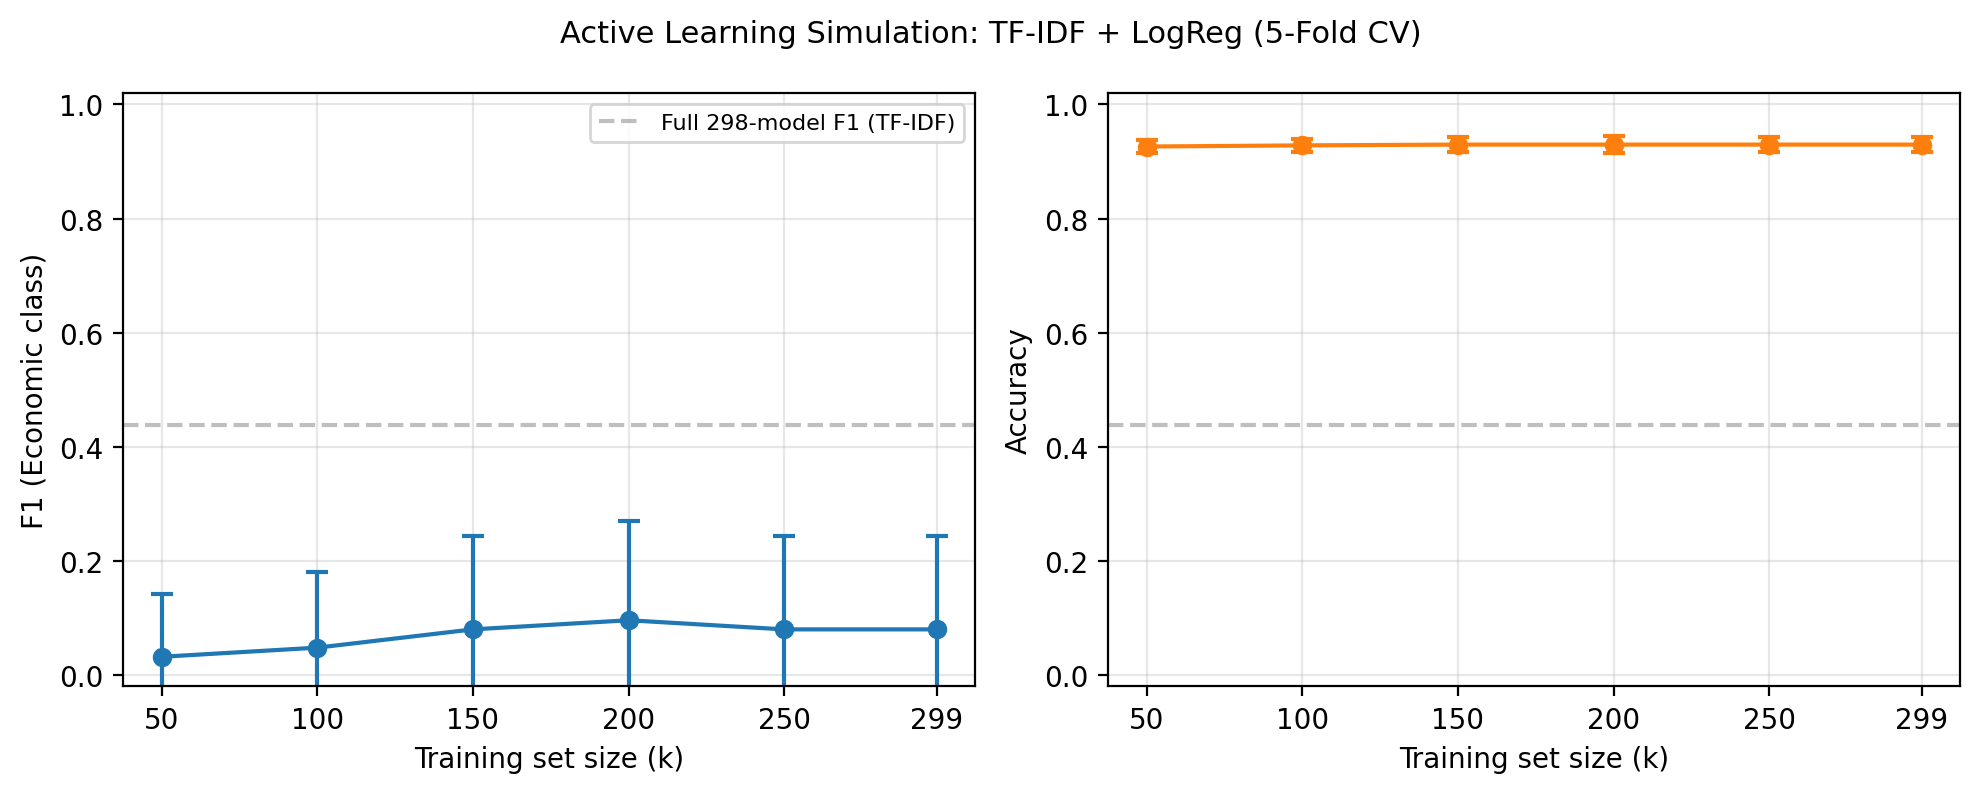
\includegraphics[width=\textwidth]{../../data/annotations/active_learning_plot.png}
\caption{Legacy active learning simulation: F1 (Economic class) and accuracy vs. annotation budget $k$. Error bars show $\pm1$ standard deviation across 25 trials. The gray dashed line marks the full-data TF-IDF F1 of 0.44. Accuracy hovers at $\sim$93\% at every budget---the majority-class baseline---while F1 never exceeds 0.10.}
\label{fig:active-learning}
\end{figure}

The curve is flat. At every budget from $k = 50$ to $k = 299$, accuracy remains at the majority-class baseline ($\sim$93\%), and F1 for the Economic class never exceeds 0.10. The classifier defaults to ``Not Economic'' for the vast majority of test articles at every budget, reflecting the fundamental difficulty of learning a minority class from 3--18 positive training examples at a 7.4\% base rate.

This result is informative as a \textit{lower bound}: with 299 articles and 22 positives, even TF-IDF---our best weak-label model---cannot overcome the base-rate problem. The minimum viable annotation budget for rare-event economic text classification with linear classifiers is substantially larger than $k = 300$, or requires a stronger model (e.g., the LLM annotator itself) or a designed sampling strategy (e.g., uncertainty sampling or positive-unlabeled learning).

\subsection{Correlation with Macroeconomic Indicators}

Table~\ref{tab:correlations} reports the relationship between the prototype monthly BENI calibration index and two key macroeconomic indicators for Bangladesh: the BDT/USD exchange rate and the CPI.

\begin{table}[h]
\centering
\begin{tabular}{lcccc}
\toprule
 & \multicolumn{2}{c}{Level} & \multicolumn{2}{c}{First-differenced} \\
\cmidrule(lr){2-3} \cmidrule(lr){4-5}
Indicator & $r$ & $p$ & $r$ & $p$ \\
\midrule
BDT/USD exchange rate & $-$0.72 & $<$0.001 & 0.10 & 0.38 \\
CPI (all items) & $-$0.75 & $<$0.001 & $-$0.04 & 0.73 \\
\bottomrule
\end{tabular}
\caption{Pearson correlations between the prototype monthly BENI calibration index and macroeconomic indicators. Level correlations are strong and negative; first-differenced correlations are negligible and statistically insignificant.}
\label{tab:correlations}
\end{table}

The level correlations ($-$0.72 with FX, $-$0.75 with CPI) indicate long-run co-movement in the calibration window: the prototype economic-news share declines over 2014--2020 while the exchange rate and consumer-price index trend upward. This pattern is useful for measurement validation, but it should not be interpreted as causal evidence or as out-of-sample forecasting performance.

The first-differenced correlations, however, are statistically indistinguishable from zero ($r = 0.10$, $p = 0.38$ for FX; $r = -0.04$, $p = 0.73$ for CPI). This means month-to-month changes in the prototype economic-news share do not predict month-to-month changes in exchange rates or consumer prices. We interpret this null result as evidence that economic narrative salience may be a long-run measurement signal rather than a short-run forecasting signal. Section~\ref{sec:discussion} examines this distinction in detail.

\paragraph{Lead correlations.} Leading BENI by 1, 3, and 6 months against the macro indicators produces similar level correlations ($r$ between $-$0.72 and $-$0.74, all $p < 0.001$), reflecting the same trend co-movement rather than predictive lead-lag relationships.


% Paper 3 — Discussion Section
% Building Local-Language Economic Narrative Indices

\section{Discussion}\label{sec:discussion}

\subsection{\texorpdfstring{The $\kappa$ Paradox}{The kappa Paradox}: Why High Accuracy Does Not Imply Reliable Classification}

On the frozen BENI v1 validation set, the repaired TF-IDF model achieves 88.17\% accuracy, 0.736 $\kappa$, and 0.823 F1 on the Economic class. The majority-class baseline still reaches 62.90\% accuracy, which is why accuracy alone remains an incomplete metric on imbalanced text classification: the more important question is how well the model recovers the minority Economic class.

The practical implication is that models must be evaluated on $\kappa$ or F1 for the minority class, not accuracy. The TF-IDF model's F1 of 0.823 on the frozen BENI v1 validation set is the operative production baseline for the repaired release. Researchers building similar indices should pre-register F1 (Economic class) or $\kappa$ as their primary metric, not accuracy.

\subsection{Why Short-Run Correlations Are Null}

The strong level correlations ($-$0.72 to $-$0.75) and null first-differenced correlations ($-$0.04 to 0.10) in the calibration experiment suggest that economic narrative salience in Bangladeshi news may operate primarily as a \textit{long-run structural} measurement signal rather than a \textit{short-run cyclical} forecasting signal.

Three interpretations are consistent with this pattern:

\begin{enumerate}
    \item \textbf{Structural transformation}: Between 2014 and 2020, Bangladesh's economy underwent significant structural change: income rose, the garment sector expanded, and digital financial services proliferated. The declining share of economic news in the calibration index may reflect a genuine shift in news composition as the economy diversified beyond headline economic stories.
    \item \textbf{News production dynamics}: Bangladeshi newspapers may allocate front-page space to economic narratives only during periods of acute economic stress or major policy events, producing a low-frequency signal that correlates with the level of macroeconomic indicators but not their monthly changes.
    \item \textbf{Nominal vs. real signal}: The level correlations may partly reflect nominal trends (both the exchange rate and consumer prices rose steadily over the period), and differencing removes this shared trend, revealing the absence of a short-run relationship.
\end{enumerate}

This null result is a methodological contribution in itself: it demonstrates that \textbf{classification improvement does not guarantee correlation improvement}. A hypothetical model that achieves very high F1 on economic relevance classification would not necessarily produce first-differenced correlations above $|r| = 0.10$, because the mapping from classification accuracy to time-series predictive power is mediated by the frequency, magnitude, and timing of narrative shifts. This finding echoes the broader sentiment forecasting literature, where publication bias inflates reported correlations~\citep{nabil2026economic}. For BENI v1, the practical implication is that the final source-balanced index must be validated separately after regeneration from the harmonised database.

\subsection{Qualitative Error Analysis}

The LLM annotator's self-consistency evaluation (Section~\ref{sec:methods}) identified 2 disagreements in 50 articles ($\kappa = 0.48$). Both cases illuminate the boundary of what constitutes ``economic relevance'' for BENI:

\begin{itemize}
    \item \textbf{Political party funding} (article \texttt{bnlp\_dev\_1208}): A debate about funding sources for political campaigns was classified as Not Economic on the first pass (focusing on the political dimension) but Economic on the second pass (focusing on the fiscal policy implications of campaign finance). The article contains economic vocabulary (budget, funding, allocation) but the primary frame is political. This suggests that borderline articles occupy a genuine grey zone where even consistent annotators disagree.
    \item \textbf{Mobile phone discounts} (article \texttt{bnlp\_train\_6027}): A report on promotional pricing by mobile operators was classified as Not Economic initially (consumer pricing, not macro-economics) but Economic on re-annotation (trade/commerce implications). The article discusses market competition and pricing strategies---microeconomic phenomena that border on trade and commerce for the BENI framework.
\end{itemize}

These disagreements are not annotator errors but genuine ambiguity at the classification boundary. They represent the irreducible uncertainty inherent in the ``Economic'' label, which no amount of annotation budget expansion or model improvement can eliminate. For the BENI pipeline, we estimate this irreducible disagreement rate at approximately 4\% (2/50), corresponding to a self-consistency ceiling of $\kappa \approx 0.48$.

\subsection{Implications for Methodology}

Three findings from this calibration study have direct implications for researchers building local-language economic narrative indices:

\begin{enumerate}
    \item \textbf{Frozen validation clarifies the production baseline.} The repaired TF-IDF model performs substantially better than the majority baseline on the frozen 186-row BENI v1 validation set, so it is the production comparator for the current release. The legacy BanglaBERT calibration result remains useful as prototype evidence, but it is not part of the frozen release tables.
    \item \textbf{Accuracy is a misleading metric for imbalanced economic text.} With base rates of 5--10\% (typical for economic relevance classification), accuracy is dominated by majority-class performance. Researchers should report $\kappa$ or minority-class F1 as their primary evaluation metric.
    \item \textbf{Active learning with linear classifiers has limited value below $k = 300$ annotations at low base rates.} The flat active learning curve shows that TF-IDF cannot learn the minority class from fewer than 300 articles with a 7.4\% positive rate. At these sample sizes, the annotation budget is better spent on acquiring higher-quality labels (e.g., through LLM annotation or uncertainty-guided sampling) than on training increasingly complex models on the same small set.
\end{enumerate}

\subsection{Implications for BENI v1}

The BENI v1 database changes the scale and purpose of the pipeline. The calibration experiment establishes the measurement logic, but the final BENI v1 index should be generated from the harmonised 1.47-million-record database with explicit source balancing, duplicate handling, and versioned model outputs. This matters because a high-volume source can dominate raw article-weighted monthly averages, and because post-2020 BNAD coverage extends the period into a different macroeconomic regime.

The next methodological step is therefore mechanical but important: freeze the annotation set, choose the production classifier, run predictions over the deduplicated BENI v1 article file, construct article-weighted and source-balanced monthly indices, and rerun the validation tables. Only after that step should the index be used in the subsequent macroeconomic validation or inflation-nowcasting papers.


% Paper 3 — Replicable Pipeline Template
% Section 7: How to build a local-language economic narrative index

\section{Replicable Pipeline Template}\label{sec:template}

This section provides a step-by-step guide for researchers who want to build a local-language economic narrative index in another language or country context. The template is designed around a single binding constraint: \textbf{the annotation budget}, measured in both time and cost.

\subsection{Step-by-Step Protocol}

\begin{enumerate}
    \item \textbf{Select a corpus.} Identify a publicly available or scrapable news corpus in the target language with at least 50,000 articles and publication dates. Sources: academic repositories (Mendeley, Zenodo), news API archives, or custom scrapers (Newspaper3k, Scrapy). \textit{Time: 1--2 weeks. Cost: \$0 if using existing corpus; \$50--\$200 for API access.}

    \item \textbf{Define the classification task.} Economic relevance is a binary label (Economic / Not Economic). For more granular tasks (sentiment, topic, narrative frame), adapt the six-field schema from Appendix~\ref{app:annotation-prompt}. Pre-register the annotation protocol and evaluation metrics (primary: F1 for the target class; secondary: Cohen's $\kappa$). \textit{Time: 1 day.}

    \item \textbf{Generate weak labels.} Create keyword-derived pseudo-labels using a domain-specific term list (see Appendix~\ref{app:keywords} for the Bangla economics term list). Expect precision of 5--45\% depending on keyword quality. This step requires no annotation budget and provides training data for the initial classifier. \textit{Time: 2--3 days. Cost: \$0.}

    \item \textbf{Train a baseline classifier.} Use TF-IDF + Logistic Regression (no GPU required). This establishes the reproducibility baseline and reveals the weak-label ceiling before any annotation budget is committed. \textit{Time: 30 minutes. Cost: \$0. Compute: 1 CPU core.}

    \item \textbf{Generate silver-standard labels.} Use an LLM annotator (Claude, GPT-4o) at temperature 0.0 with a structured prompt to annotate 300--500 articles. Self-consistency check on 50 articles. Total API cost at current rates: \$1--\$5 for 300 articles. \textit{Time: 1--2 days. Cost: \$1--\$5. Compute: None (API).}

    \item \textbf{Evaluate the weak-label ceiling.} Compare the TF-IDF baseline against the silver standard. Compute McNemar's test between any two weak-label models to determine whether architectural improvements extract additional signal. If $p > 0.05$, the weak labels are the binding constraint. \textit{Time: 1 hour.}

    \item \textbf{Decide on annotation investment} (see Section~\ref{sec:investment-decision} below). If the weak-label F1 is below 0.5 and resources permit, invest in designed sampling (uncertainty-guided, not random) for the next annotation batch. \textit{Time: varies.}

    \item \textbf{Build the index.} Aggregate monthly scores, compare article-weighted and source-balanced specifications, preserve model and release versions, and validate against available macroeconomic indicators. \textit{Time: 1--2 days after predictions are complete.}
\end{enumerate}

\subsection{Cost Table}\label{sec:cost-table}

Table~\ref{tab:costs} summarizes the compute and financial costs associated with each step, using the BENI pipeline as a reference.

\begin{table}[h]
\centering
\small
\begin{tabular}{lccc}
\toprule
Component & Compute & Time & Cost (USD) \\
\midrule
Corpus acquisition & 1 CPU, 4 GB RAM & 1--2 weeks & \$0--\$200 \\
Keyword weak labels & 1 CPU & 2--3 days & \$0 \\
TF-IDF + LogReg training & 1 CPU, 2 GB RAM & 2 minutes & \$0 (free tier) \\
LLM annotation (300 articles) & API only & 1--2 days & \$1--\$5 \\
Self-consistency check (50 articles) & API only & 1 hour & \$0.20--\$1 \\
Transformer fine-tuning (100k--1M articles) & 16 GB GPU (T4) & 2--8 hours & \$0 (Kaggle) or \$2--\$10 \\
McNemar + evaluation & 1 CPU & 1 minute & \$0 \\
Active learning simulation & 1 CPU, 4 GB RAM & 30 minutes & \$0 \\
Index construction and validation & 1 CPU & 10--60 minutes & \$0 \\
\bottomrule
\end{tabular}
\caption{Compute and cost estimates for each pipeline step. Total: \$3--\$208, primarily corpus-dependent.}
\label{tab:costs}
\end{table}

The total pipeline cost---excluding corpus acquisition---is **under \$10** for the LLM annotation (300 articles) and can be as low as **\$3** when free API credits or open-source models are used. The compute requirements are met by any consumer laptop with 8 GB RAM for the TF-IDF stages; only the BanglaBERT fine-tuning step requires a GPU (available at no cost via Kaggle or Google Colab).

\subsection{Annotation Investment Decision Tree}\label{sec:investment-decision}

Figure~\ref{fig:decision-tree} presents a decision tree for determining the minimum viable annotation investment based on the target base rate and available resources. The key thresholds, derived from the BENI experiments, are:

\begin{itemize}
    \item \textbf{Base rate $\geq$ 20\%}: Random sampling of 200--300 articles with TF-IDF + LogReg achieves F1 $\geq$ 0.6. LLM annotation is optional.
    \item \textbf{Base rate 10--20\%}: Active learning with uncertainty sampling reaches 90\% of full performance at $k \approx 250$. LLM annotation recommended.
    \item \textbf{Base rate $<$ 10\%} (BENI case): Random sampling fails at all budgets up to $k = 300$. Designed sampling (uncertainty-guided, positive-unlabeled learning) or LLM annotation is essential. Minimum budget: $k \geq 500$ for TF-IDF, or $k \geq 200$ with LLM-generated labels.
\end{itemize}

\begin{figure}[h]
\centering
\begin{tabular}{ll}
\toprule
Situation & Recommended Action \\
\midrule
No budget, no API access & Keyword weak labels + TF-IDF baseline only \\
\$5--\$10 budget, base rate $<$ 10\% & LLM annotate 300 articles, TF-IDF evaluation \\
\$10--\$50 budget & LLM annotate 300--500 + designed sampling \\
GPU available (free tier) & Add BanglaBERT fine-tuning on weak labels \\
Human annotators available & 2 annotators $\times$ 300 articles + adjudication \\
\bottomrule
\end{tabular}
\caption{Decision matrix for annotation strategy by budget and setting.}
\label{fig:decision-tree}
\end{figure}

\subsection{Validation Checklist}

Before publishing an index, verify each item on the following checklist:

\begin{enumerate}
    \item \textbf{Annotation reliability}: Report Cohen's $\kappa$, observed agreement, and prevalence-adjusted $\kappa$ for the annotation set.
    \item \textbf{Model ceiling}: Compare against a TF-IDF baseline on identical training labels. Report McNemar's test.
    \item \textbf{Active learning curve}: Report F1 (target class) vs. annotation budget across at least 5 budget levels with confidence intervals.
    \item \textbf{Temporal validation}: Use temporal train/val/test splits (not random). Report performance separately for each period.
    \item \textbf{Macro correlation}: Report both level and first-differenced correlations with at least two independent macroeconomic indicators.
    \item \textbf{Source balance}: Report article-weighted and source-balanced indices, especially when source volume is uneven.
    \item \textbf{Reproducibility}: Publish all code, annotation prompts, and preprocessed data files.
\end{enumerate}


% Paper 3 — Conclusion
% Building Local-Language Economic Narrative Indices

\section{Conclusion}\label{sec:conclusion}

We presented the BENI v1 method pipeline, a reproducible workflow for transforming Bangla-language newspaper articles into economic narrative measurements. The paper contributes a harmonised database design, a weak-label and LLM-assisted annotation strategy, a frozen validation protocol, and a reproducible article-level prediction and monthly index pipeline for local-language news.

On the frozen BENI v1 validation set, the repaired TF-IDF model achieves 88.17\% accuracy and 0.823 F1 on the Economic class. That is the production baseline for the current release. The majority baseline remains much weaker on the minority class, which confirms that the index still depends on a genuinely trained classifier rather than a trivial threshold rule.

The monthly BENI v1 index now exists in frozen form with article-weighted and source-balanced variants. The prototype Potrika calibration index still reveals strong long-run co-movement with macroeconomic indicators, but those prototype results are separated from the frozen release tables. Improved classification accuracy does not automatically translate to better short-run prediction, so the next validation papers should treat the frozen index as a measurement object before using it for forecasting.

For BENI v1, the current paper now supplies the frozen empirical base for later macroeconomic validation and nowcasting work.

\subsection{Limitations}

This study has five main limitations. First, the silver standard uses LLM-generated labels rather than human expert annotations. While the self-consistency check ($\kappa = 0.48$, 96\% agreement) provides a reliability ceiling, true gold-standard validation requires human annotators. Second, the clean frozen validation set is only 186 articles (69 Economic), limiting the precision of downstream comparisons. Third, the prototype macro-validation results use the older Potrika calibration index, not the final frozen BENI v1 index. Fourth, the time series used in the calibration analysis covers only 79 months (2014--2020), which is sufficient for long-run correlation but insufficient for robust out-of-sample forecasting evaluation. Fifth, the analysis is limited to Bangladesh---generalizability to other low-resource languages and economies remains to be tested.

\subsection{Future Work}

Three directions follow directly. First, human annotation of a larger set (1,000+ articles) would enable true gold-standard validation and more precise active learning estimates. Second, validating the frozen BENI v1 index on the extended sample will test source-balanced narrative indicators against the broader macroeconomic series. Third, incorporating the frozen BENI v1 index into a nowcasting framework for Bangladesh inflation---as outlined in the broader research program---would test whether the long-run narrative signal can be combined with high-frequency official statistics for real-time economic monitoring.


\paragraph{Acknowledgments.}
The author thanks the anonymous developers of the Potrika corpus and the BNLP dataset for making Bangla NLP research possible.

\bibliographystyle{plainnat}
\bibliography{references}

\appendix
\section{Annotation Prompt}\label{app:annotation-prompt}

The full annotation prompt used for Claude Sonnet 4 is available in the supplementary materials and the GitHub repository (\url{https://github.com/ann-nabil/economic-narrative-indices}).

\section{Economic Keyword List}\label{app:keywords}

The full list of 32 Bangla economic terms used for keyword-based pseudo-label generation is available in the supplementary materials.

\end{document}
